% \input{\pathsections "sec discussion"}

\section{Backup}

%%  %%  %%  %%  %%
\subsection{The Best Fit May be Crap}
%
\begin{frame}\frametitle{Nature Choses the Functional Form}
	%
	The Best Fit May be Crap.
	%
\end{frame}
%
%
%\subsection{Anscombe's Devilish Data Set}
\newcommand{\myscale}[0] {0.60}

\begin{frame}
\frametitle{\quartet \ I}
%
\begin{table}[htbp]
%\caption[Anscombe's data set quartet]{Anscombe's data set quartet. Despite glaring dissimilarities, each data set present the same solution.}
	\begin{center}
	\begin{tabular}{ccc}
			%
			%
	Data set 1 && Data set 2 \\
	\begin{overpic}[ scale = \myscale ]
		{\pLocalGraphics anscombe-01-blue-data-v-fit}
			% 
		\put(6,10){\colorbox{white}{\bl{\anscombe}}}
			%
	\end{overpic}
	&&
	\begin{overpic}[ scale = \myscale ]
		{\pLocalGraphics anscombe-02-blue-data-v-fit}
		\put(6,10){\colorbox{white}{\bl{\anscombe}}}
	\end{overpic} \\
			%
			%
	\end{tabular}
	\end{center}
\label{tab:anscombe-data-set-error}
\end{table}%
\end{frame}
%
\begin{frame}
\frametitle{\quartet \ II}
%
\begin{table}[htbp]
%\caption[Anscombe's data set quartet]{Anscombe's data set quartet. Despite glaring dissimilarities, each data set present the same solution.}
	\begin{center}
	\begin{tabular}{ccc}
			%
	Data set 3 && Data set 4 \\
	\begin{overpic}[ scale = \myscale ]
		{\pLocalGraphics anscombe-03-blue-data-v-fit}
			% 
		\put(6,10){\colorbox{white}{\bl{\anscombe}}}
			%
	\end{overpic}
	&&
	\begin{overpic}[ scale = \myscale ]
		{\pLocalGraphics anscombe-04-blue-data-v-fit}
		\put(6,10){\colorbox{white}{\bl{\anscombe}}}
	\end{overpic}
			%
	\end{tabular}
	\end{center}
\label{tab:anscombe-data-set-error-ii}
\end{table}%
\end{frame}
%
\begin{frame}
\frametitle{\quartet \ I}
%
\begin{table}[htbp]
%\caption[Anscombe's data set quartet]{Anscombe's data set quartet. Despite glaring dissimilarities, each data set present the same solution.}
	\begin{center}
	\begin{tabular}{ccc}
			%
			%
	Data set 1 && Data set 2 \\
	\begin{overpic}[ scale = \myscale ]
		{\pLocalGraphics anscombe-01-residuals}
			% 
		%\put(6,10){\colorbox{white}{\bl{\anscombe}}}
			%
	\end{overpic}
	&&
	\begin{overpic}[ scale = \myscale ]
		{\pLocalGraphics anscombe-02-residuals}
		%\put(6,10){\colorbox{white}{\bl{\anscombe}}}
	\end{overpic} \\
			%
			%
	\end{tabular}
	\end{center}
\label{tab:anscombe-data-set-error}
\end{table}%
\end{frame}
%
\begin{frame}
\frametitle{\quartet \ II}
%
\begin{table}[htbp]
%\caption[Anscombe's data set quartet]{Anscombe's data set quartet. Despite glaring dissimilarities, each data set present the same solution.}
	\begin{center}
	\begin{tabular}{ccc}
			%
			%
	Data set 3 && Data set 4 \\
	\begin{overpic}[ scale = \myscale ]
		{\pLocalGraphics anscombe-03-residuals}
			% 
		%\put(6,10){\colorbox{white}{\bl{\anscombe}}}
			%
	\end{overpic}
	&&
	\begin{overpic}[ scale = \myscale ]
		{\pLocalGraphics anscombe-04-residuals}
		%\put(6,10){\colorbox{white}{\bl{\anscombe}}}
	\end{overpic} \\
			%
			%
	\end{tabular}
	\end{center}
\label{tab:anscombe-data-set-error}
\end{table}%
\end{frame}
%
\begin{frame}
\frametitle{Least Squares Does Not}
\begin{enumerate}
	\item Legitimize a bad model
	\item Turn bad data into good results
\end{enumerate}
\end{frame}
%
\begin{frame}
\frametitle{Least Squares Does}
\begin{enumerate}
	\item Provide \bl{quantitative} data for model \bl{comparison}
	\item Provide \bl{best fit} for the chosen model
\end{enumerate}
\end{frame}
%
%
\subsection{Why Least Squares?}

\subsubsection{Norms}
\begin{frame}\frametitle{\href{https://mathworld.wolfram.com/VectorNorm.html}{Vector Norms}}
	%
	Norms quantify \bl{length} and \bl{proximity}.
	%
\end{frame}
%
%
\begin{frame}
\frametitle{The Continuum of $p$ norms}
$$1 \le p < \infty$$
$$ \normp{x} = \paren{\abs{x_{1}}^{1/p} + \abs{x_{2}}^{1/p} + \dots + {\abs{x_{m}}^{1/p}}}^{1/p} $$ 
\end{frame}
%
%
\begin{frame}\frametitle{Norms as Path Length}
	%
\center
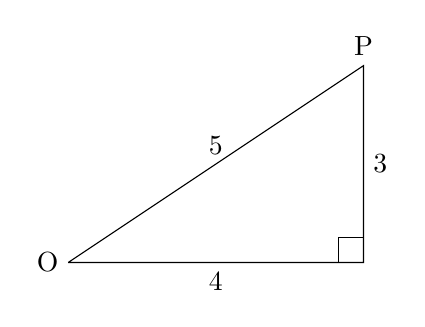
\begin{tikzpicture}[scale=1.25]%,cap=round,>=latex]

\coordinate [label=left:O] (A) at (-1.5cm,-1.cm);
\coordinate [label=right:] (C) at (1.5cm,-1.0cm);
\coordinate [label=above:P] (B) at (1.5cm,1.0cm);
\draw (A) -- node[above] {$5$} (B) -- node[right] {$3$} (C) -- node[below] {$4$} (A);

\draw (1.25cm,-1.0cm) rectangle (1.5cm,-0.75cm);

\end{tikzpicture}
	%
\end{frame}
%
%
\begin{frame}\frametitle{Popular $p$ norms}
	%
\begin{equation}
	\begin{array}{lll}
			%
		\normo{p} &= \abs{x} + \abs{y} &= 7 \\[5pt]
			%
		\normt{p} &= \sqrt{x^{2} + y^{2}} &= 5 \\[5pt]
			%
		\normi{p} &= \max\paren{\abs{x}, \abs{y}} &= 4
			%
	\end{array}
\end{equation}
	%
\end{frame}
%
%
\begin{frame}
\frametitle{The Unit Circle in Different Norms}
$$\normp{x+y} = 1$$
\begin{table}[htp]
%\caption{default}
\begin{center}
\begin{tabular}{ccc}
		%
	$p=1$ & $p=2$ & $p=\infty$ \\
		%
	\includegraphics[ width = 1.25 in ]{\pLocalGraphics norm-1-c2} &
		%
	\includegraphics[ width = 1.25 in ]{\pLocalGraphics norm-2-c2} &
		%
	\includegraphics[ width = 1.25 in ]{\pLocalGraphics norm-inf-c2} \\
		%
\end{tabular}
\end{center}
\label{tab:norms}
\end{table}%
\end{frame}%
\begin{frame}
\frametitle{Why Use $\normt{\cdot}$: Incorrect Answers}
\begin{enumerate}
	\item Herd instinct
	\item Peer pressure
	\item Precedent
\end{enumerate}
\end{frame}
%
\begin{frame}
\frametitle{Why Use $\normts{\cdot}$: Correct Answers}
\begin{enumerate}
	\item \href{https://en.wikipedia.org/wiki/Gauss\%E2\%80\%93Markov_theorem}{Gauss--Markov Theorem}
	\item Differentiability
\end{enumerate}
\end{frame}
%
\subsection{The Normal Equations}
%
%
\begin{frame}\frametitle{The Normal Equations in Numeric Computation}
\begin{center}
	\begin{overpic}[ scale = 0.70 ]
		{\pLocalGraphics scream-02}
		\put(15, 85)	{\colorbox{white}{Noooooooo!}}
	\end{overpic} \\
\end{center}
\end{frame}
%
%
\begin{frame}\frametitle{The Normal Equations in Numeric Computation}
	%
\begin{table}[htp]
%\caption{default}
\begin{center}
\begin{tabular}{ll}
		%
	system & condition number \\\hline
	\ \\
		%
	$\axeb$ & $\kappa_{2}(\A{}) = \displaystyle\frac{\sigma_{1}} {\sigma_{n}}$  \\[10pt]
		%
	 $\AsA \, x = \A{*}b$ &
		$\kappa_{2}(\A{}) = \displaystyle\paren{\frac{\sigma_{1}} {\sigma_{n}}}^\rd{{2}}$
		%
\end{tabular}
\end{center}
%\label{default}
\end{table}%
	%
\end{frame}
%
%
\begin{frame}\frametitle{The Normal Equations in Numeric Computation}
	%
	\center
Noisy problems become \rd{unsolvable}
	%
\end{frame}
%
\begin{frame}\frametitle{The Normal Equations in Numeric Computation}
	%
	Linear system with 3-digit arithmetic\footnote{Meyer, Example 4.5.1}
	%
\begin{equation}
	\A{} = \mat{ll}{3 & 6 \\ 1 & 2.01}, \quad b= \mat{l}{9 \\ 3.01} 
\end{equation}
	%
\begin{equation}
	\xls = \mat{c}{1 \\ 1} 
\end{equation}
	%
\end{frame}
%
\begin{frame}\frametitle{The Normal Equations in Numeric Computation}
	%
	Normal equations are \rd{singular}\footnote{e.g. row 2 = 2 $\times$ row 1}
	%
\begin{equation}
	\AsA{} = \mat{cc}{10 & 20 \\ 20 & 40} 
\end{equation}
	%
\end{frame}
%
\subsubsection{The Normal Equations in Theory}
\begin{frame}\frametitle{The Normal Equations in Theory}
	%
	$$\AsA x =  \A{*}b$$
	%
\begin{enumerate}
	\item Always consistent
	\item For $\rho = n$, solution is \bl{unique}
	\item For $\rho = n$, solution is $\bl{\xls} = \Anormal b$
\end{enumerate}
	%
\end{frame}
%
\begin{frame}\frametitle{The Normal Equations in Theory}
	%
Proof: Equivalence of \\ 
	$x_{N}$, \bl{normal equations solution} and \\
	$\xls$, \bl{least squares solution}
	%
	%
\end{frame}
%
\begin{frame}\frametitle{The Normal Equations in Theory}
	%
Proof: Outline
\begin{table}[htp]
%\caption{default}
\begin{center}
\begin{tabular}{lll}
		%
	$1$ & $t^{2}= \normts{\A{}\xls - b}$ & definition \\[5pt]
	\pause
	$2$ & $\A{}x_{N} - \A{}x_{N}$ & propitious zero \\[5pt]
	\pause
	$3$ & $t^{2}= \normts{\A{}\xls \mg{+ \A{}x_{N} - \A{}x_{N}} - b}$ & restatement of 1 \\[5pt]
	\pause
	$4$ & $t^{2} \rd{\le} \normts{A{}x_{N} - b} + \normts{\A{}\paren{\xls -x_{N}}}$ & triangle inequality \\[5pt]
	\pause
	$5$ & $...$ & \bl{Miracle}\\[5pt]
	\pause
	$6$ & $t^{2} \bl{=} \normts{A{}x_{N} - b} + \normts{\A{}\paren{\xls -x_{N}}}$ & target (Pythagoras)\\[5pt]
	\pause
	$7$ & $t^{2} = t^{2} + \normts{\A{}\paren{\xls -x_{N}}}$ & evaluation\\[5pt]
	\pause
	$8$ & $\normts{\A{}\paren{\xls -x_{N}}} = 0$ & conclusion\\
		%
\end{tabular}
\end{center}
%\label{default}
\end{table}%
	%
\end{frame}

%%  %%  %%  %%  %%
\subsection{Notation}
%
\begin{frame}\frametitle{Notation Options}
	%
Examples of notation 
\begin{enumerate}
	\item Inner product form
	\item Vector form
	\item Scalar form
\end{enumerate}
\end{frame}
%
%
\begin{frame}\frametitle{Exact Solution Notation: Inner Products}
	%
\begin{equation}
	\bl{a_{p}} = \bl{ \bevSolnI } 
\tag{\ref{eq:bevSolnC}}
\end{equation}
	%
\begin{equation}
	\Delta = \bl{ \bevDetI } 
\tag{\ref{eq:bevdeterminant}}
\end{equation}

\end{frame}
%
\begin{frame}\frametitle{Exact Solution Notation: Vectors}
	%
\begin{equation}
	\bl{a_{p}} = \bl{ \bevSolnV } 
\tag{\ref{eq:bevSolnC}}
\end{equation}
	%
\begin{equation}
	\Delta = \bl{ \bevDetV } 
\tag{\ref{eq:bevdeterminant}}
\end{equation}
\end{frame}
%
\begin{frame}\frametitle{Exact Solution Notation: Scalar Form}
\begin{equation}
	\bl{a_{p}} = \bl{ \bevSolnC } 
\tag{\ref{eq:bevSolnC}}
\end{equation}
	%
\begin{equation}
	\Delta = \bl{ \bevDetC } 
\tag{\ref{eq:bevdeterminant}}
\end{equation}
\end{frame}


%%  %%  %%  %%  %%
\subsection{Bounding Errors}
\begin{frame}\frametitle{Data, Fit, Result, Residuals}
\begin{center}
		\begin{overpic}[ scale = 1.0 ]
			{\pLocalGraphics bev-error-good-red}
			\put(10, 55){$T_{LS}(x) = 4.81389 + 9.40833x $}
			%\put(10, 50)	{\colorbox{white}{$\littleap = \bevSolnNumeric \pm \bevErrorNumeric$}}
			%\put(10, 40)	{\colorbox{white}{$t^{2} \approx 317 $}}
			\labelx
			\labelT 
		\end{overpic}  \\[20pt]
\end{center}
\end{frame}

\begin{frame}\frametitle{Data, Fit, Result, Residuals}
\begin{center}
		\begin{overpic}[ scale = 1.0 ]
			{\pLocalGraphics bev-error-good-red}
			\put(10, 55){$T_{LS}(x) = (4.8 \pm 4.9 ) + (9.41 \pm 0.87 )x $}
			%\put(10, 50)	{\colorbox{white}{$\littleap = \bevSolnNumeric \pm \bevErrorNumeric$}}
			%\put(10, 40)	{\colorbox{white}{$t^{2} \approx 317 $}}
			\labelx
			\labelT 
		\end{overpic}  \\[20pt]
\end{center}
\end{frame}
%
\begin{frame}\frametitle{Data, Fit, 1 $\sigma$ Error}
\begin{center}
	\begin{overpic}[ scale = 1.0 ]
		{\pLocalGraphics bevington-data-soln-bands}
		%\put(10, 50){$T_{LS}(x) = (4.8 \pm 4.9 ) + (9.41 \pm 0.87 )x $}
		\put(7,45){\colorbox{white}{$T_{\bl{+}}(x)= \paren{a_{0} \bl{+} \sigma_{0}} + \paren{a_{1} \bl{+} \sigma_{1}} x$}}
		\put(38,15){\colorbox{white}{$T_{\rd{-}}(x)= \paren{a_{0} \rd{-} \sigma_{0}} + \paren{a_{1} \rd{-} \sigma_{1}} x$}}
		\labelx
		\labelT
	\end{overpic}  \\[20pt]
\end{center}
\end{frame}
%
%
\endinput  %  ==  ==  ==  ==  ==  ==  ==  ==  ==
